% !TEX root = ../my-thesis.tex
%

% -------------------------------------------

\chapter{The Complete Maximum a Posteriori Method}
\label{sec:cmp}

\cleanchapterquote{Sire, je n'avais pas besoin de cette hypoth\`ese.}{Pierre Simon de Laplace}{(French Mathematician, 1749-1827)}

\section{Introduction}
\label{sc:cmp:intro}

This section introduces the \gls{cmp} method. The goal is to provide practitioners with a modular approach to perform model calibration that can accurately approximate the marginal posterior distribution of the parameters, $\p{\btheta \mid \data}$. The \gls{cmp} method therefore retains the best features of both worlds, i.e.,

\begin{enumerate}
    \item It is a modular approach based on the adaptive estimation of the hyperparameters, $\psimap$, as a function of the parameters.
    \item It reduces the dimensionality of the calibration problem by separating the hyperparameters' and parameters' estimation problems.
    \item It approximates the parameters' marginal posterior distribution, $\p{\btheta \mid \data}$, without the need to compute a possibly high-dimensional integral.
\end{enumerate}

This method is based on the following idea: instead of approximating the parameters' marginal posterior distribution by evaluating the joint posterior distribution at a fixed value of the hyperparameters, as in the \gls{koh} method, we can evaluate the joint posterior distribution along a curve, $c(\btheta) = \left(\btheta, \psimap\right)$, where $\psimap$ is the value of the hyperparameters that maximizes the joint distribution $\p{\btheta, \bpsi \mid \data}$ for each value of the parameters, $\btheta$. This approach is similar to the \gls{fmp} method, but it differs from it in the final expression of the parameters' marginal posterior distribution, which, as will be shown in the rest of this section, includes the prior distribution of the hyperparameters and a correction factor that accounts for the uncertainty in the estimation of $\psimap$.

\smallskip
The main intuition for the \gls{cmp} approach is based on the relationship between three objects, namely the joint posterior distribution, $\p{\btheta, \bpsi \mid \data}$, the parameters' marginal posterior distribution, $\p{\btheta \mid \data}$, and the hyperparameters' conditional distribution, $\p{\bpsi \mid \btheta, \data}$. These objects are connected by the rule of marginal probabilities,

\begin{equation}
    \p{\btheta, \bpsi \mid \data} = \p{\btheta \mid \data} \ \p{\bpsi \mid \btheta, \data} \;.
    \label{eq:cmp:hpar_posterior}
\end{equation}

The joint distribution $\p{\btheta, \bpsi \mid \data}$ is known up to a normalization constant while the parameters' marginal posterior distribution, $\p{\btheta \mid \data}$, is the quantity we want to approximate. The hyperparameters' conditional distribution, $\p{\bpsi \mid \btheta, \data}$, is the key object that allows us to connect the joint distribution and the parameters' marginal posterior distribution. In fact, if we can find a functional relationship between the hyperparameters and the parameters by using $\p{\bpsi \mid \btheta, \data}$, we can evaluate the joint distribution along a curve defined by this functional relationship and obtain an approximation of the parameters' marginal posterior distribution.

\smallskip
To build some intuition we start by considering the case in which the hyperparameters' marginal distribution is a Gaussian distribution with a mean that depends on the parameters, $\psimap$, and a covariance matrix that depends on the parameters, $\boldsymbol{\Sigma}_{\btheta}$, i.e., $\p{\bpsi \mid \btheta, \data} = \mathcal{N}(\bpsi; \psimap, \boldsymbol{\Sigma}_{\btheta})$. In this case, evaluating the joint distribution along the curve defined by $\psimap$ returns the following expression,

\begin{equation}
    \normalpdf(\psimap; \psimap, \boldsymbol{\Sigma}_{\btheta})  = \dfrac{1}{\sqrt{(2\pi)^d \abs{\detf{\boldsymbol{\Sigma}_{\btheta}}}}} \;.
    \label{eq:intuition}
\end{equation}

Eq.~\eqref{eq:intuition} shows that evaluating the conditional distribution at its maximum value, $\psimap$, returns a constant that depends on the covariance matrix, $\boldsymbol{\Sigma}_{\btheta}$. If we multiply this expression by the joint distribution evaluated at $\psimap$, we are performing an operation that is equivalent to integrating the hyperparameters' conditional distribution over the hyperparameters' space, i.e.,

\begin{equation}
    \p{\psimap \mid \btheta, \data} \sqrt{(2\pi)^d \abs{\detf{\boldsymbol{\Sigma}_{\btheta}}}} = 1 = \intpsi{\p{\bpsi \mid \btheta, \data}} \;.
    \label{eq:cmp:intuition_2}
\end{equation}

By combining Eq.~\eqref{eq:cmp:hpar_posterior} and Eq.~\eqref{eq:cmp:intuition_2} we see that the act of marginalizing the joint distribution over the hyperparameters, which is the operation that allows us to obtain the parameters' marginal posterior distribution, can be approximated by evaluating the joint distribution along a curve defined by $\psimap$ and by multiplying it by a correction factor, $\sqrt{(2\pi)^d \abs{\detf{\boldsymbol{\Sigma}_{\btheta}}}}$, 

\begin{equation}
    \p{\btheta \mid \data} = \intpsi{\p{\btheta, \bpsi \mid \data}}  =  \p{\btheta, \psimap \mid \data}  \sqrt{(2\pi)^d \abs{\detf{\boldsymbol{\Sigma}_{\btheta}}}}  \;.   
\end{equation}

In the remainder of this section, we are going to formalize the intuition presented above into the core of the \gls{cmp} method. We shall see that the Gaussian assumption is not necessary to obtain a closed-form expression of the parameters' marginal posterior distribution, and that what we need is to postulate that the hyperparameters' conditional distribution changes its shape only by some scaling and shifting as the parameters change. We are also going to show that the correction factor, $\sqrt{(2\pi)^d \abs{\detf{\boldsymbol{\Sigma}_{\btheta}}}}$, is connected to the Hessian of the posterior distribution at its maximum value in the hyperparameters. The \gls{cmp} method is therefore a generalization of the Laplace approximation.

\smallskip
The remainder of this section is organized as follows. In \S\ref{sc:cmp:assumptions} we present the assumptions of the \gls{cmp} method. In \S\ref{sc:cmp:par_post} we show how to obtain a closed-form expression of the parameters' marginal posterior distribution. In \S\ref{sc:cmp:pred_post} we present an approximation of the predictive posterior distribution of the corrected model. In \S\ref{sc:cmp:sc_fact} we show how to compute the correction factor. In \S\ref{sc:cmp:el_examples} we present two elementary examples to illustrate the application of the \gls{cmp} method and to show its advantages over the \gls{koh} and \gls{fmp} methods. The examples in \S\ref{sc:cmp:examples} show the application of the \gls{cmp} method to more complex calibration problems. This chapter is taken from a contribution published in the \textit{International Journal for Uncertainty Quantification}~\cite{cmp}.

\section{Assumptions of the CMP Method}
\label{sc:cmp:assumptions}

Here we present the assumptions upon which the \gls{cmp} method relies. These assumptions are crucial to simplify the integration of the hyperparameters and to obtain a closed-form expression of the parameters' marginal posterior distribution. 

\smallskip
First and foremost, we assume that the hyperparameters' conditional distribution, $\p{\bpsi \mid \btheta, \data}$, has a unique global maximum value, $\psimap \in \Psi$, for each possible value of the parameters, $\btheta$. This maximum value is defined as,

\begin{equation}
    \psimap = \argmax_{\bpsi \in \Psi} \p{\bpsi \mid \btheta, \data} = \argmax_{\bpsi \in \Psi} \p{\btheta, \bpsi \mid \data} \;.
    \label{eq:cmp:psi_map}
\end{equation}

This assumption is well justified in the context of model calibration. In fact, the hyperparameters are typically related to the model error and the experimental error noise, and it is reasonable to expect that there is a unique value of these quantities that maximizes the posterior distribution. Interestingly, the \gls{koh} estimation of the hyperparameters is intimately related to the \gls{cmp} estimation. Recall that the \gls{koh} estimation of the hyperparameters is defined as,

\begin{equation}
   \psikoh = \argmax_{\bpsi \in \Psi} \, \int_{\Theta} \p{\btheta, \bpsi \mid \data} \, \mathrm{d}\btheta \;.
\end{equation}

Using the definition of the \gls{cmp} method, Eq.~\eqref{eq:cmp:hpar_posterior}, we can rewrite the \gls{koh} estimation as follows,

\begin{equation}
    \left.
        \begin{aligned}
    \psikoh &=  \argmax_{\bpsi \in \Psi} \, \mathbb{E}_{\btheta \sim \p{\btheta \mid \data}}\left[ \ \p{\bpsi \mid \btheta, \data} \ \right]\\
    &=   \mathbb{E}_{\btheta \sim \p{\btheta \mid \data}}\left[ \ \argmax_{\bpsi \in \Psi} \ \p{\bpsi \mid \btheta, \data} \ \right] \\
    & = \expectation{\btheta \sim \p{\btheta \mid \data}}{\psimap} \;.
        \end{aligned}
    \right.
    \label{eq:koh_hpar}
\end{equation}

The \gls{koh} value of the hyperparameters is the posterior-averaged value of the functional relationship between the hyperparameters and the parameters introduced by the \gls{fmp} method. 

\smallskip 
Our second assumption is that the conditional distribution $\p{\bpsi \mid \btheta, \data}$ can be approximated by a fixed distribution, $s : \Phi \rightarrow \mathbb{R}^+$, which we call \textit{shape function}. The conditional distribution and the shape function are connected via an affine transformation 

\begin{equation}
    \bphi = \Stheta (\bpsi - \psimap) \;.
    \label{eq:cmp:linear_transform}
\end{equation}

The transformation matrix $\Stheta$ must be invertible. Therefore,

\begin{equation}
    \p{\bpsi \mid \btheta, \data} \approx s(\bphi) \, \abs{\detf{\Stheta}} \;.
    \label{eq:cmp:hp_cmp}
\end{equation}

These hypotheses correspond to requiring that the hyperparameters' conditional distribution, as $\btheta$ changes, changes its shape only by some scaling and shifting. 

\begin{figure}[htbp]
        \centering 
        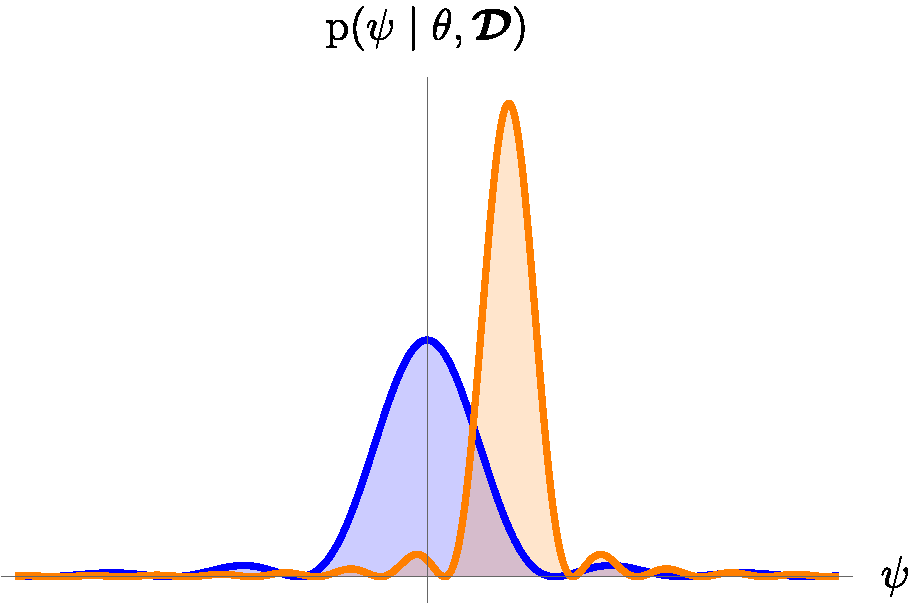
\includegraphics[width=0.6\textwidth]{figures/cmp/fig_1.pdf}
        \caption{Example (sketch) of a consistent hyperparameters' conditional distribution for two values of the parameters (blue and orange curves).}
        \label{fig:cmp:fig_1}
\end{figure}

In Fig.~\ref{fig:cmp:fig_1} we report a sketch of a consistent hyperparameters' conditional distribution for two values of the parameters (blue and orange curves). Here the shape function is $s(\phi)\propto \mathrm{sinc}^2(\phi)$, and we have chosen this example to stress the fact that, although the function can have multiple local maxima, the global maximum should be unique. As visible in the figure, the affine transformation corresponds to some shifting and scaling of the shape function.
We recall that if the shape function is a point mass distribution, $s(\bphi)=\delta(\bphi)$, the \gls{cmp} method reduces to the \gls{fmp} method (with uniform prior).
Moreover, if $s(\bphi) = \dfrac{1}{\sqrt{2\pi}}\ \exp - \dfrac{\bphi^{\top} \ \bphi}{2}$, we recover the Laplace approximation. 

In any case, computing the shape function is not necessary for the computation of the \gls{cmp} approximation of the marginal posterior distribution, and we only need to postulate its existence. We anticipate, however, that for the computation of the predictive posterior distribution, the shape function must be known, and we are going to present a further approximation to avoid computing it in \S\ref{sc:cmp:pred_post}.

\section{Computation of the Marginal Posterior}
\label{sc:cmp:par_post}

The parameters' posterior distribution is defined as the marginalization of the joint posterior distribution over the hyperparameters. To avoid the computation of a possibly high-dimensional integral, we can use the assumptions of the \gls{cmp} method to obtain a closed-form expression of the parameters' marginal posterior distribution. Starting from Eq.~\eqref{eq:cmp:hpar_posterior} and using the second hypothesis of the \gls{cmp} method, defined in Eq.~\eqref{eq:cmp:hp_cmp}, we can write

\begin{equation}
    \p{\psimap \mid \btheta, \data} \dfrac{1}{\abs{\detf{\Stheta}}} \approx s(\boldsymbol{0})  \; .
    \label{eq:cmp:cmp_0}
\end{equation}

We can therefore multiply the left and right-hand sides of Eq.~\eqref{eq:cmp:cmp_0} by the parameters' marginal posterior distribution, $\p{\btheta \mid \data}$, and obtain

\begin{equation}
    \left.
        \begin{aligned}
            \p{\btheta \mid \data} s(\boldsymbol{0}) &\approx \p{\btheta \mid \data} \  \p{\psimap \mid \btheta, \data} \ \dfrac{1}{\abs{\detf{\Stheta}}}\\
            &= \p{\btheta, \psimap \mid \data} \ \dfrac{1}{\abs{\detf{\Stheta}}}\;.
        \end{aligned}
    \right.
    \label{eq:cmp_1}
\end{equation}

This means that marginalizing the joint distribution over the hyperparameters, a procedure that previously required the evaluation of a possibly high-dimensional integral, can now be done by evaluating the joint distribution along a curve, $c(\btheta)=\left(\btheta, \psimap\right)$, and dividing by a \textit{correction factor}, $\abs{\detf{\Stheta}}$. We can now use Bayes's theorem to express the joint distribution in terms of the likelihood and the prior distribution, and obtain the following expression for the parameters' marginal posterior distribution,

\begin{equation}
    \mathrm{p}_{_\cmp} (\btheta \mid \data) \propto \likelihood{\data \mid  \btheta, \psimap} \ \prior{\btheta} \ \prior{\psimap} \ \dfrac{1}{\abs{\detf{\Stheta}}}\; .
    \label{eq:cmp:cmp}
\end{equation}

The expression still relies on the availability of $\abs{\detf{\Stheta}}$ whose expression is discussed in \S\ref{sc:cmp:sc_fact}. One can immediately see that, contrary to the \gls{fmp} method, the \gls{cmp} method evaluates both the likelihood and the prior distribution of the hyperparameters on $\psimap$. This is a crucial difference as the prior distribution of the hyperparameters can be informative and can influence the parameters' marginal posterior distribution. Furthermore, dividing by the correction factor, $\abs{\detf{\Stheta}}$, ensures that the \gls{cmp} distribution correctly recovers the parameters' marginal distribution.

\subsection{Approximation of the Predictive Posterior}
\label{sc:cmp:pred_post}

We now turn to the question of approximating the predictive distribution of the model error term at a new input location $\bx$, i.e. $\p{z(\bx) \mid \data}$. In the \gls{fb} framework, the computation of this quantity required the evaluation of an integral over the parameters and the hyperparameters, see Eq.~\eqref{eq:sota_1:z_pred}. In the \gls{cmp} method, a posterior distribution of the hyperparameters is not available, and we need to approximate it using our estimate of the hyperparameters, $\psimap$. Starting from the definition of the predictive distribution of the model error term, we can write,

\begin{equation}
    \left.
        \begin{aligned}
            \p{z \mid \data} &= \intt{\intpsi{\p{z \mid \btheta, \bpsi, \data} \ \p{\btheta, \bpsi \mid \data}}} \\
            & \text{Using Eq.~\eqref{eq:cmp:hpar_posterior}, } \\
            &= \intt{ \p{\btheta \mid \data} \ \intpsi{\p{z \mid \btheta, \bpsi, \data} \ \p{ \bpsi \mid \btheta, \data}}}\\
            & \text{From Eq.~\eqref{eq:cmp:hp_cmp},} \\
            &\propto \intt{ \p{\btheta \mid \data} \ \intpsi{\p{z \mid \btheta, \bpsi, \data} \ s\left(\bphi \right) \abs{\detf{\Stheta}}}} \\
            & \text{ Using Eq.~\eqref{eq:cmp:linear_transform}}\\
            & = \intt{ \p{\btheta \mid \data}} \ \intphi{\p{z \mid \btheta, \psimap + \Stheta^{-1} \bphi, \data} \ s(\bphi)} \;.
        \end{aligned}
    \right.
    \label{eq:cmp:pred_base}
\end{equation}

We introduce the following abbreviation for the argument of the integral,

\begin{equation}
    \left.
    \begin{aligned}
        \argp{\cmp}{z \mid \btheta} &= \intphi{\p{z \mid \btheta, \psimap + \Stheta^{-1} \bphi} \ s(\bphi)}\\
        & = \expectation{\bphi \sim s(\bphi)}{\p{z \mid \btheta, \psimap + \Stheta^{-1} \bphi}} \;.
    \end{aligned}
    \right.
\label{eq:cmp:arg_pred}
\end{equation}


This integral cannot be evaluated without an explicit expression for the shape function, $s(\bphi)$, preventing direct sampling from $\p{z \mid \data}$. To address this issue, we propose to return to a point-wise approximation, by assuming that the shape function is a point mass distribution, $s(\bphi) = \delta(\bphi)$,


\begin{equation}
    \approxp{_\cmp}{ z \mid \btheta, \data} = \p{z \mid \btheta, \psimap, \data} \; .
    \label{eq:cmp:corr_pred}
\end{equation}

The proposed approximation, Eq.~\eqref{eq:cmp:corr_pred}, can be evaluated using the \glspl{gp} predictive equations \cite{gp_rasmussen}, reported in \S\ref{sec:ntools:gpr}. The result can then be averaged over the parameters' marginal posterior distribution, Eq.~\eqref{eq:cmp:cmp}, to obtain the predictive distribution of the corrected model, 

\begin{equation}
    \p{z \mid \data} \approx \intt{\approxp{_\cmp}{ z \mid \btheta, \data} \ \mathrm{p}_{_\cmp} (\btheta \mid \data)} \;.
    \label{eq:cmp:pred}
\end{equation}

On the one hand, introducing the point mass distribution assumption neglects the uncertainty of the hyperparameters and makes Eq.~\eqref{eq:cmp:pred} overconfident. On the other hand, the uncertainty of the hyperparameters is already accounted for in the parameters' marginal posterior distribution which is used in Eq.~\eqref{eq:cmp:pred} to average Eq.~\eqref{eq:cmp:corr_pred}. This means that the \gls{cmp} predictive distribution, although not exact, is still an improvement over the \gls{fmp} predictive distribution.

\subsection{Evaluation of the Correction Factor}
\label{sc:cmp:sc_fact}

The \gls{cmp} method relies on the availability of the correction factor, $\abs{\detf{\Stheta}}$, which, as of now, was not specified. We can however show that this quantity is connected to the Hessian of the posterior distribution at its maximum value in the hyperparameters. This is firstly done by substituting the hypothesis of the \gls{cmp} method, Eq.~\eqref{eq:cmp:hp_cmp}, in the log of Eq.~\eqref{eq:cmp:hpar_posterior}:

\begin{equation}
    \boldsymbol{\nabla}^2_{\bpsi} \;\log \p{\btheta, \psimap \mid \data} \approx \boldsymbol{\nabla}^2_{\bpsi} \; \log s (\boldsymbol{0}) \;.
\end{equation}

Using the chain rule we obtain

\begin{equation}
    \boldsymbol{\nabla}^2_{\bpsi} \; \log s (\boldsymbol{0}) = \Stheta^{\top} \ \mathbf{H}_0 \ \Stheta \; ,
\end{equation}

where $\mathbf{H}_0=\boldsymbol{\nabla}^2_{\bphi} \ \log s(\boldsymbol{0})$ is a constant matrix equal to the Hessian of the log of the shape function at the origin. By the properties of the determinant, 

\begin{equation}
    \sqrt{\abs{\detf{\boldsymbol{\nabla}^2_{\bpsi} \;\log \p{\btheta, \psimap \mid \data}}}} \propto \abs{\detf{\Stheta}} \;.
    \label{eq:cmp:det_jac}
\end{equation}

The Hessian of the posterior distribution is available in closed form provided that the derivatives of the model error's covariance function and the log-prior are available. Numerical differentiation techniques can be used to compute these derivatives for different types of likelihood and prior functions. On the other hand, in the case in which the likelihood is Gaussian, we can obtain a closed-form expression of its gradients. To see this, recall the expression of the log-likelihood for a Gaussian likelihood,

\begin{equation}
    \log \likelihood{\data \mid \btheta, \bpsi} = -\dfrac{1}{2} \log \abs{\detf{\mathbf{K}_{\bpsi}}} - \dfrac{1}{2} \bres^{\top} \mathbf{K}_{\bpsi}^{-1} \bres + C \;,
     \label{eq:cmp:ll}
\end{equation}

Where $\bres = (y_i - f(\mathbf{x}_i; \btheta))^T_{i=1\ldots n}$ is the vector of residuals, $\mathbf{K}_{\bpsi} = k_{\bpsi}(\mathbf{X}, \mathbf{X}) + \boldsymbol{\Sigma}_e$ is the covariance matrix of the observations, and $C$ is a constant that does not depend on $\btheta$ and $\bpsi$. We can now take the derivative of the log-likelihood with respect to the hyperparameters, $\psi_k$, and obtain the following expression~\cite{gp_rasmussen},


\begin{equation}
     \partial_{\psi_k} \log \likelihood{\data \mid \btheta, \bpsi} = \mathrm{Tr}{\dfrac{1}{2} (\balpha \balpha^{\top} - \mathbf{K}_{\bpsi}^{-1}) \  \dfrac{\partial \mathbf{K}_{\bpsi}}{\partial \psi_k}} \; ,
     \label{eq:cmp:ll_gradient}
\end{equation}

with $\balpha = \mathbf{K}_{\bpsi}^{-1} \bres$. We proceed by taking the derivative a second time and by using the fact that the trace operator is linear,

\begin{equation}
\left.
    \begin{aligned}
        \partial_{\psi_l} \partial_{\psi_k} \log \likelihood{\data \mid \btheta, \bpsi}  = & \dfrac{1}{2} \ \mathrm{Tr}\left((\balpha \balpha^{\top} - \mathbf{K}^{-1}_{\bpsi})\dfrac{\partial^2 \mathbf{K}_{\bpsi}}{\partial \psi_l \partial \psi_k}\right)  \\
        & + \dfrac{1}{2}\ \mathrm{Tr}\left(\dfrac{\partial \balpha \balpha^{\top}}{\partial \psi_l} \dfrac{\partial \mathbf{K}_{\bpsi}}{\partial \psi_k} \right) \\
        & - \dfrac{1}{2}\ \mathrm{Tr} \left(\dfrac{\partial \mathbf{K}_{\bpsi}^{-1}}{\partial \psi_l} \dfrac{\partial \mathbf{K}_{\bpsi}}{\partial \psi_k}\right) \;.
    \end{aligned}
\right.
\label{eq:cmp:hess_ll_1}
\end{equation}

Eq.~\eqref{eq:cmp:hess_ll_1} shows that the Hessian of the log-likelihood is the sum of three contributions. 
The first contribution involves the Hessian of the observations' covariance matrix. The second contribution can be simplified in the following way: 

\begin{equation}
    \left.
    \begin{aligned}
            & \dfrac{\partial \balpha \balpha^{\top}}{\partial \psi_l} = 2 \ \text{Sym} \left( \dfrac{\partial \balpha}{\partial \psi_l} \balpha^{\top} \right) \; , \\
            & \frac{\partial \balpha}{\partial \psi_l}  = \frac{\partial \mathbf{K}_{\bpsi}^{-1}}{\partial \psi_l} \bres = -\mathbf{K}_{\bpsi}^{-1} \dfrac{\partial \mathbf{K}_{\bpsi}}{\partial \psi_l} \mathbf{K}_{\bpsi}^{-1} \bres \; .
    \end{aligned}
    \right.
    \label{eq:cmp:hess_ll_2}
\end{equation}

The third contribution can be simplified by using similar arguments.
To simplify the notation, we proceed by defining $\mathbf{A}_i = \mathbf{K}_{\bpsi}^{-1} \dfrac{\partial \mathbf{K}_{\bpsi}}{\partial \psi_i}$. Combining Eq.~\eqref{eq:cmp:hess_ll_2} and Eq.~\eqref{eq:cmp:hess_ll_1} yields

\begin{equation}
\left.
    \begin{aligned}
        \partial_{\psi_l} \partial_{\psi_k} \log \likelihood{\data \mid \btheta, \bpsi} = \ & \dfrac{1}{2} \ \mathrm{Tr}\left((\balpha \balpha^{\top} - \mathbf{K}^{-1}_{\bpsi}) \; \dfrac{\partial^2 \mathbf{K}_{\bpsi}}{\partial \psi_l \ \partial \psi_k}\right)  \\
        & - \mathrm{Tr}\left( \text{Sym} \left( \mathbf{A}_l \ \balpha \balpha^{\top} \right) \; \dfrac{\partial \mathbf{K}_{\bpsi}}{\partial \psi_k}\right) \\
        & + \dfrac{1}{2} \mathrm{Tr}\left( \mathbf{A}_l  \mathbf{A}_k\right)\,.
    \end{aligned}
\right.
\label{eq:cmp:hess_ll}
\end{equation}

The Hessian of the log-likelihood with respect to the hyperparameters can be cheaply evaluated provided that the covariance and its gradients are known and that the inverse of the covariance matrix is available. 

\section{Elementary Examples}
\label{sc:cmp:el_examples}

In this section, we present two elementary examples to illustrate the application of the \gls{cmp} method and show its advantages over the \gls{koh} and \gls{fmp} methods. Both examples are chosen because they can be solved analytically, giving valuable insights into the method. The first example, in \S\ref{sc:cmp:no_model_err_cal}, is a calibration problem in which the model is well-specified. The second one, in \S\ref{sc:cmp:mix_gauss}, is a calibration problem in which the true posterior distribution is a mixture of Gaussian distributions with well-separated modes.

\subsection{Example 1: Calibration of a Well-Specified Model}
\label{sc:cmp:no_model_err_cal}

In this example, we consider the calibration of a well-specified model. We recall that a well-specified model is a model that can perfectly fit the observations, i.e. there exists a value of the parameters, $\btheta^\star$, such that the computer code $f(\bx; \btheta^\star)$ can perfectly reproduce the observations, $\mathbf{y}$. 

\smallskip
As an elementary example, this setting is not particularly interesting for practical applications. However, it is useful to illustrate the application of the \gls{cmp} method and to show that it can recover the true parameters' marginal posterior distribution and how the \gls{koh} and \gls{fmp} methods fail to do so.

\smallskip
Under this assumption, the model error term reduces to zero, and the only source of uncertainty is the experimental error noise, $\epsilon$. The calibration equation is therefore defined as follows,

\begin{equation}
    \mathbf{y} = f(\mathbf{X}; \btheta) + \epsilon \;.
\end{equation}

Further assuming that the experimental error noise is Gaussian with zero mean and variance $\sigma_e^2$, the likelihood function is defined as follows,

\begin{equation}
    \likelihood{ \data \mid \btheta, \sigma_e} = \dfrac{1}{\displaystyle\sqrt{(2\pi \sigma_e^2)^{\nobs}}} \, \exp{\left(-\dfrac{\rr}{2\sigma_e ^2}\right)} \;. 
\end{equation}


Concerning the prior distribution of the experimental error noise, $\prior{\sigma_e}$, we choose an improper power law prior distribution with parameter $a>0$,

\begin{equation}
    \prior{\sigma_e} = \dfrac{1}{\sigma_e^a} \; .
\end{equation}

If $a=0$ we recover a uniform prior distribution, if $a=1$ we recover a log-uniform prior distribution and if $a=2$ we recover Jeffrey's prior. The solution is reported as a function of the parameter $a$. Under this setting, the hyperparameters' conditional distribution, $\p{\sigma_e \mid \btheta, \data}$, can be computed in closed form by using Bayes's theorem and by marginalizing the joint distribution over the parameters. We obtain,

\begin{equation}
    \left.
        \begin{aligned}
            \p{\sigma_e \mid \btheta, \data} &= \dfrac{\p{\btheta, \sigma_e \mid \data}}{\displaystyle \int_{0}^{\infty} \p{\btheta, \sigma_e \mid \data} \ \dd \sigma_e} \\
            &\propto\dfrac{1}{\sqrt{\rr}} \
            e^{-\dfrac{ \rr }{2 \sigma_e
            ^2}}
            \left(\dfrac{\sqrt{\rr}}{\sigma_e
            }\right)^{\nobs+a}\; .
        \end{aligned}
    \right.
    \label{eq:cmp:cmp_noerr}
\end{equation}

We can compute $\sigma_e^{_\map}$ and $\abs{\detf{S_{\btheta}}}$ by following Eq.~\eqref{eq:cmp:psi_map} and Eq.~\eqref{eq:cmp:det_jac} respectively. We obtain,

\begin{equation}
    \left.
    \begin{aligned}
        &\sigma_e^{_\map} \left( \btheta \right) = \sqrt{\dfrac{\rr}{\nobs+a}} \;,\\
        &\abs{\detf{S_{\btheta}}} = \sqrt{2 \ \dfrac{a+\nobs}{\rr}}  \propto \sqrt{\dfrac{1}{\rr}}\;.\\
    \end{aligned}
    \right.
    \label{eq:cmp:sigma_e_map}
\end{equation}

Calling $t = \dfrac{\sigma_e}{\sqrt{\rr}}$ and by using Eq.~\eqref{eq:cmp:sigma_e_map}, we can rewrite Eq.~\eqref{eq:cmp:cmp_noerr} as

\begin{equation}
    \p{\sigma_e \mid \btheta, \data} \propto \; \abs{\detf{S_{\btheta}}} \, e^{-\dfrac{1}{2 t^2}} \,
    \left(\dfrac{1}{t}\right)^{\nobs+a}\; .
    \label{eq:cmp:cmp_noerr_1}
\end{equation}

We can recover the affine transformation by noting that

\begin{equation}
    \phi = S_{\btheta} \left( \sigma_e - \sigma_e^{_\map} \right) = t - \sqrt{\frac{1}{\nobs+a}} = t - \phi_0\;.
    \label{eq:cmp:phi_nme}
\end{equation}

Finally, substituting Eq.~\eqref{eq:cmp:phi_nme} in Eq.~\eqref{eq:cmp:cmp_noerr_1} it yields

\begin{equation}
    \p{\sigma_e \mid \btheta, \data} \propto \; \abs{\detf{S_{\btheta}}} \, e^{-\dfrac{1}{2 (\phi+\phi_0)^2}} \,
    \left(\dfrac{1}{\phi+\phi_0}\right)^{\nobs+a}\; .
    \label{eq:cmp:cmp_noerr_2}
\end{equation}

As it is possible to see, Eq.~\eqref{eq:cmp:cmp_noerr_2} respects exactly the hypothesis of the \gls{cmp} method. Since all quantities are available in closed form, we can directly compute the shape function, $s(\phi)$, by using Eq.~\eqref{eq:cmp:hp_cmp},
\begin{equation}
    \left.
    \begin{aligned}
        s(\phi) &: (-\phi_0, \infty) \rightarrow \mathbb{R}^+ \;,\\
        &\propto e^{-\dfrac{1}{2 (\phi+\phi_0)^2}} \,
        \left(\dfrac{1}{\phi+\phi_0}\right)^{\nobs+a} \;.
    \end{aligned}
    \right.
\end{equation}

\begin{figure}[htbp]
    \centering 
    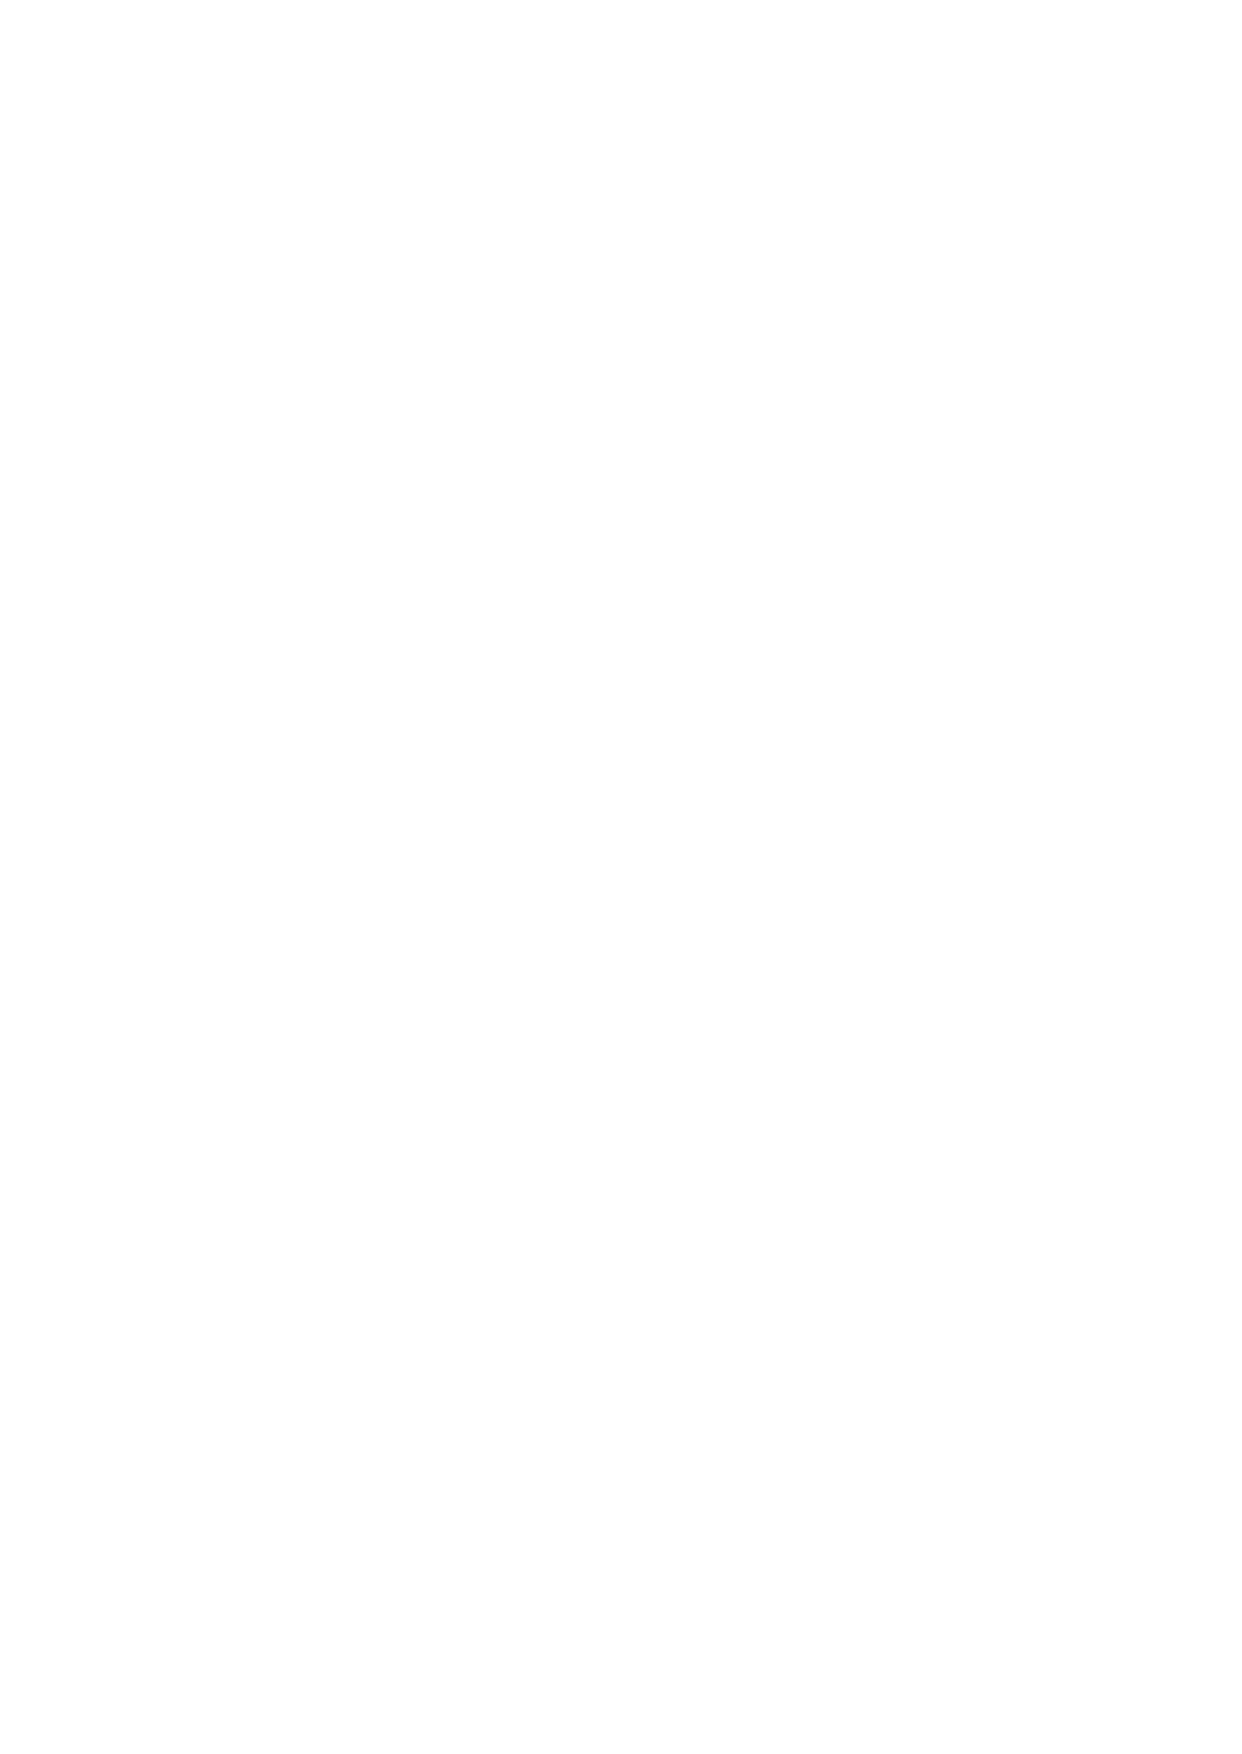
\includegraphics[width=0.6\textwidth]{figures/cmp/fig_2.pdf}
    \caption{Shape function.}
    \label{fig:cmp:fig_2}
\end{figure}

Fig.~\ref{fig:cmp:fig_2} depicts the shape function for the \gls{cmp} calibration problem with no model error choosing $\nobs+a=10$. In this case, the \gls{cmp} approximation will yield the exact result.

\smallskip
The correction factor, given in Eq.~\eqref{eq:cmp:sigma_e_map}, is crucial in this case. Omitting it would lead to a parameter's posterior distribution that overemphasizes areas where the residuals are small and underemphasizes areas where the residuals are large. Since large residuals are typically found in the tails of the distributions, the correction factor is essential to prevent the false certainty effect.


\subsection{Example 2: Mixture of Gaussians}
\label{sc:cmp:mix_gauss}

In this subsection, we assess the \gls{cmp} approximation of the parameters' marginal posterior distribution in the case where the posterior distribution is a mixture of Gaussian distributions with well-separated modes. 

\smallskip
This example is particularly interesting because it tackles a common situation in model calibration, i.e. the presence of multiple modes in the posterior distribution. In fact, the posterior distribution can be multimodal for different reasons, such as the presence of multiple local maxima in the likelihood function or the presence of symmetries in the model. The presence of multiple modes can lead to a false certainty effect if not properly accounted for, and it is therefore crucial to have a method that can correctly approximate the parameters' marginal posterior distribution in this case. It is well-known that the \gls{koh} method is unable to correctly capture every mode of the posterior distribution, and it is therefore expected that the \gls{cmp} method will outperform the \gls{koh} method in this case. On the other hand, the \gls{fmp} method can capture every mode of the posterior distribution but it cannot correctly estimate the importance of each mode, leading to a false certainty effect. 


\smallskip
We consider the case in which the joint posterior, $\p{\boldsymbol{\gamma}=(\btheta,\bpsi) \mid \data}$, is a mixture of $M$ Gaussian distributions with weights $w_i : \summ{i}{1}{M} w_i =1$, means $\boldsymbol{\mu}_i = \begin{pmatrix} \boldsymbol{\mu}_{\btheta,i} \\ \boldsymbol{\mu}_{\bpsi,i} \end{pmatrix}$, and covariance matrices $\mathbf{K}_i = \begin{bmatrix}
    \mathbf{K}_{\btheta,i} & \mathbf{K}_{\btheta,\bpsi,i} \\
    \mathbf{K}_{\btheta,\bpsi,i}^{\top} & \mathbf{K}_{\bpsi,i}
\end{bmatrix}$. The posterior distribution is given by

\begin{equation}
    \left.
        \begin{aligned}
            \p{\btheta, \bpsi \mid \data} &\propto \sum_{i=1}^{M} w_i \ \dfrac{1}{\sqrt{(2\pi)^{d_\theta + d_\psi} \ \detf{\mathbf{K}_i}}} \\
            & \exp\left( -\dfrac{1}{2}(\boldsymbol{\gamma}-\boldsymbol{\mu}_i)^{\top} \mathbf{K}_i^{-1} (\boldsymbol{\gamma}-\boldsymbol{\mu}_i)\right) \;.
        \end{aligned}
        \right.
    \label{eq:mix_gauss}
\end{equation}

We assume that the modes are well-separated. This translates into requiring that the intervals: $\Theta_i = \left\{ \btheta : (\boldsymbol{\mu}_{i, \btheta} - \btheta)^{\top} \mathbf{K}_{\btheta,i}^{-1} (\boldsymbol{\mu}_{i, \btheta} - \btheta)  \leq t_{95\%}^{d_\theta} \right\}_{i=1\ldots M}$ (with $t_{95\%}^{d_\theta}$ equal to the 95\% quantile of the $\chi_2$ law with $d_{\theta}$ degrees of freedom) are disjoint. An equivalent condition is supposed to hold for the hyperparameters. Under this hypothesis, the hyperparameters' conditional distribution can be well approximated by

\begin{equation}
    \left.
        \begin{aligned}
    \p{\bpsi \mid \btheta, \data} \approx & \, \summ{i}{1}{M} \ \mathcal{I}(\btheta \in \Theta_i) \ \dfrac{1}{\sqrt{(2\pi)^{d_\psi} \ \detf{\mathbf{K}_{\bpsi,i \mid \btheta}}}} \\
    &\exp\left( -\dfrac{1}{2}(\bpsi-\boldsymbol{\mu}_{\bpsi,i \mid \btheta})^{\top} \mathbf{K}_{\bpsi,i \mid \btheta}^{-1} (\bpsi-\boldsymbol{\mu}_{\bpsi,i \mid \btheta})\right) \;.
        \end{aligned}
    \right.
    \label{eq:hp_mix_gauss}
\end{equation}

The conditional means can be expressed as $\boldsymbol{\mu}_{\bpsi,i \mid \btheta} = \boldsymbol{\mu}_{\bpsi,i} + \mathbf{K}_{\btheta,\bpsi,i}^{\top} \mathbf{K}_{\btheta,i}^{-1} (\btheta - \boldsymbol{\mu}_{\btheta,i})$ and the conditional covariances as $\mathbf{K}_{\bpsi,i \mid \btheta} = \mathbf{K}_{\bpsi,i} - \mathbf{K}_{\btheta,\bpsi,i}^{\top} \mathbf{K}_{\btheta,i}^{-1} \mathbf{K}_{\btheta,\bpsi,i}$. The function $\mathcal{I}(\btheta \in \Theta_i)$ is the indicator function that is equal to 1 if $\btheta \in \Theta_i$ and 0 otherwise. Note that Eq.~\eqref{eq:hp_mix_gauss} holds because we assumed that the modes are well-separated and hence we can treat each mode as a separated Gaussian distribution. Furthermore, conditioning a multivariate Gaussian distribution on a subset of its variables results in a Gaussian distribution \cite{gp_rasmussen}. 

\smallskip
According to \cite{fmp} and Eq.~\eqref{eq:cmp:det_jac}, the optimal hyperparameters, $\psimap$, and the correction factor, $\abs{\detf{\Stheta}}$, are well approximated by the following piecewise constant functions

\begin{equation}
    \left.
    \begin{aligned}
        \psimap &\approx \sum_{i=1}^{M} \boldsymbol{\mu}_{\bpsi,i \mid \btheta} \ \mathcal{I}(\btheta \in \Theta_i) \;,\\
        \abs{\detf{\Stheta}} &\approx \sum_{i=1}^{M} \dfrac{1}{\sqrt{\detf{\mathbf{K}_{\bpsi,i \mid \btheta}}}} \ \mathcal{I}(\btheta \in \Theta_i) \;.
    \end{aligned}
    \right.
    \label{eq:cmp:cmp_mix_gauss}
\end{equation} 

\begin{figure}[htbp]
    \centering
    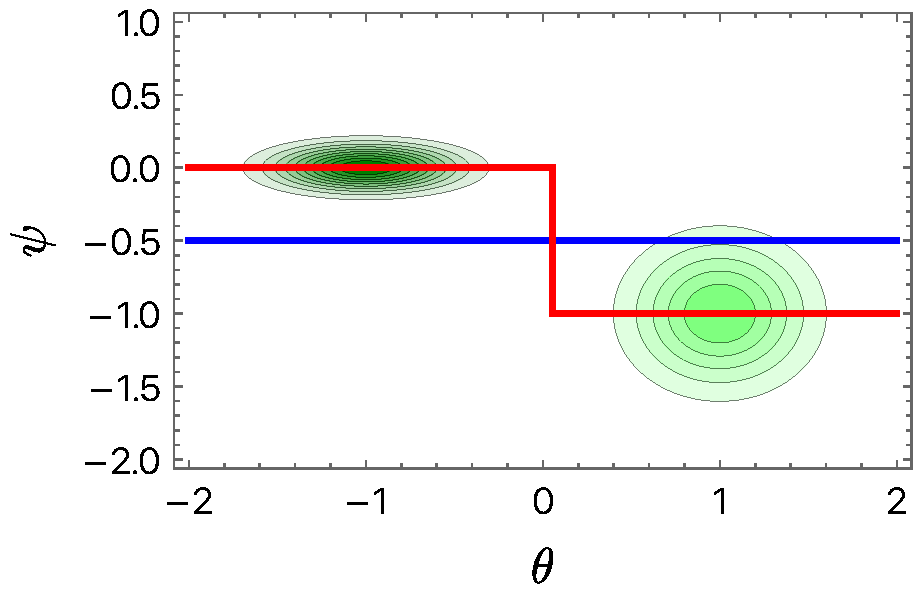
\includegraphics[width=0.6\textwidth]{figures/cmp/fig_3.pdf}
    \caption{Example of a mixture of Gaussian distribution. The red line represents the \gls{map} value of the hyperparameters, $\psimap$, and the blue line represents the \gls{koh} value.}
    \label{fig:cmp:fig_3}
\end{figure}

Fig.~\ref{fig:cmp:fig_3} shows an example of a mixture of Gaussian distribution with two modes centered in $(-1,0)$ and $(1,-1)$ respectively. The covariance matrices are diagonal with elements $(0.1,0.01)$ and $(0.1,0.1)$ respectively. The red line represents the \gls{map} value of the hyperparameters, $\psimap$, and the blue line represents the \gls{koh} value whose expression is reported in \cite{fmp}. Using the definition of the \gls{cmp} method, Eq.~\eqref{eq:cmp:cmp}, with Eq.~\eqref{eq:cmp:cmp_mix_gauss} and the hypothesis of well-separated modes, we can compute the \gls{cmp} approximation of the parameters' marginal posterior distribution,

\begin{equation}
    \left.
        \begin{aligned}
            \approxp{_\cmp}{\btheta \mid \data} &\propto \sum_{i=1}^{M} \ w_i \ \dfrac{\sqrt{\detf{\mathbf{K}_{\bpsi,i \mid \btheta}}}}{\sqrt{(2\pi)^{d_\theta + d_\psi} \ \detf{\mathbf{K}_i}}} \\
            & \exp\left( -\dfrac{1}{2}\begin{pmatrix}
                \btheta - \boldsymbol{\mu}_{\btheta,i} \\
                \boldsymbol{\mu}_{\bpsi,i \mid \btheta} - \boldsymbol{\mu}_{\bpsi,i}
            \end{pmatrix}^{\top} \mathbf{K}_i^{-1} \begin{pmatrix}
                \btheta - \boldsymbol{\mu}_{\btheta,i} \\
                \boldsymbol{\mu}_{\bpsi,i \mid \btheta} - \boldsymbol{\mu}_{\bpsi,i}
            \end{pmatrix}\right) \;.
        \end{aligned}
        \right.
    \label{eq:cmp:mix_gauss_1}
\end{equation}


We can exploit the block structure of the covariance matrix, $\mathbf{K}_{i}$, to express its determinant as $\detf{\mathbf{K}_i} = \detf{\mathbf{K}_{\btheta,i}} \detf{\mathbf{K}_{\bpsi,i \mid \btheta}}$ \cite{matrix_id}. Additionally, the argument of the exponential simplifies to $-\dfrac{1}{2} \left( \btheta - \boldsymbol{\mu}_{\btheta,i} \right)^{\top} \mathbf{K}_{\btheta,i}^{-1} \left( \btheta - \boldsymbol{\mu}_{\btheta,i} \right)$, see \cite{fmp} for the details. Introducing these simplifications in Eq.~\eqref{eq:cmp:mix_gauss_1} and normalizing the distribution yields

\begin{equation}
    \left.
        \begin{aligned}
            \approxp{_\cmp}{\btheta \mid \data} &\approx \sum_{i=1}^{m} w_i \ \dfrac{1}{\sqrt{(2\pi)^{d_\theta} \ \detf{\mathbf{K}_{\btheta,i}}}} \\
            & \exp\left( -\dfrac{1}{2} \left( \btheta - \boldsymbol{\mu}_{\btheta,i} \right)^{\top} \mathbf{K}_{\btheta,i}^{-1} \left( \btheta - \boldsymbol{\mu}_{\btheta,i} \right) \right) = \p{\btheta \mid \data} \;.
        \end{aligned}
        \right.
    \label{eq:cmp:mix_gauss_2}
\end{equation}

The expression in Eq.~\eqref{eq:cmp:mix_gauss_2} is the exact representation of the parameters' marginal posterior distribution \cite{fmp}. 

\begin{figure}[htbp]
    \centering
    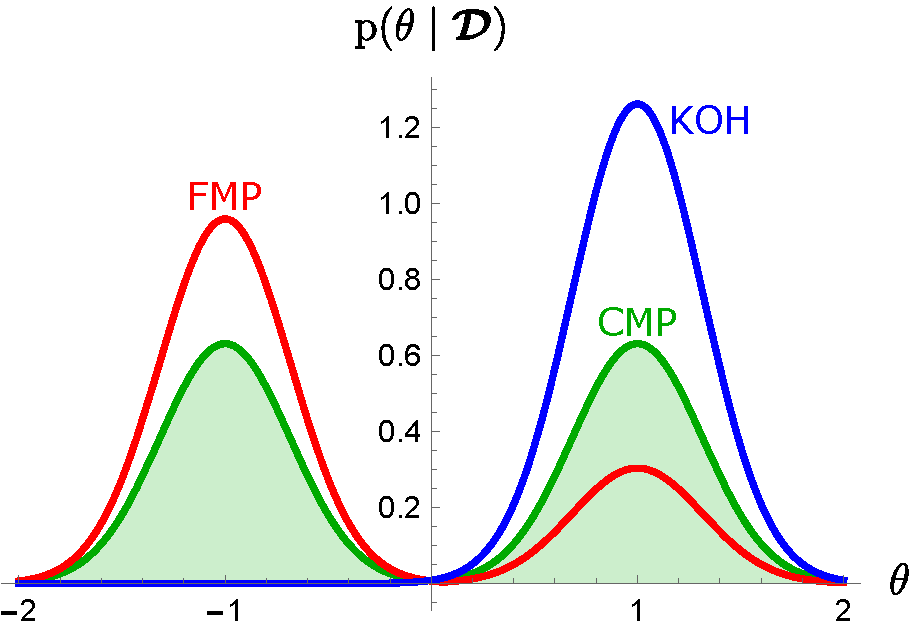
\includegraphics[width=0.6\textwidth]{figures/cmp/fig_4.pdf}
    \caption{Parameters' marginal posterior distribution.}
    \label{fig:cmp:fig_4}
\end{figure}

Fig.~\ref{fig:cmp:fig_4} shows the resulting parameters' marginal posterior distribution for the mixture of Gaussian distribution reported in Fig. \ref{fig:cmp:fig_3}. The \gls{cmp} approximation is exact and can correctly capture the modes and their weights. This is in contrast with the \gls{koh} method which can capture only a single mode and the \gls{fmp} method which can capture all the modes but misrepresents their weights. The reader is referred to \cite{fmp} for the derivation of the \gls{koh} and \gls{fmp} approximations.

\smallskip
It is important to note that the \gls{cmp} approximation is exact due to the well-separated nature of the modes. When the modes are not well-separated, the \gls{cmp} method offers an approximate marginal posterior distribution of the parameters that may not be exact. Nonetheless, we contend that the \gls{cmp} method remains preferable, as it is likely to yield a more accurate approximation compared to the \gls{koh} and \gls{fmp} methods.

\section{Examples}
\label{sc:cmp:examples}

The first example in \S\ref{sc:cmp:in_model} addresses the calibration of an inadequate model, inspired by \cite{fmp}, featuring a bimodal posterior. The results demonstrate that the \gls{cmp} method can capture both modes and their relative weights, unlike the \gls{fmp} and \gls{koh} methods. The second example, in \S\ref{sc:cmp:test_case}, involves the calibration of a problem that depends on three parameters and three hyperparameters, resulting in an unimodal posterior distribution. The novel method accurately captures the variability of this mode, leading to more robust predictions and correcting the false certitude effect characteristic of modular methods.

\subsection{Example 1: Bimodal Posterior}
\label{sc:cmp:in_model}

In this example, the true function is $y(x) = x$. 
The experimental data consists of 11 synthetically generated observations, equally spaced within the interval [0,1], based on the true model with the addition of white noise, $\epsilon \sim \normalpdf (0,0.01^2)$.

The computer model, which is an inadequate representation of the real process, depends on a single parameter called $\theta$. The computer model is defined in Eq.~\eqref{eq:cmp:stat_model}, where the measurement error is modeled as a white noise process $\epsilon \sim \normalpdf (0,\sigma_e^2)$ and the model error is represented by a \gls{gp} with zero mean and a \gls{rbf} covariance:

\begin{equation}
    \left.
    \begin{aligned}
        & \text{Computer model: } & f(x;\theta) = (1-\theta ) (x+0.15)+x \sin (2 \theta  x) \\
        & \text{Model error covariance: } &  \gpcov (x,x^{\prime}) = \sigma^2 \exp{-\dfrac{1}{2} \left(\dfrac{x-x^{\prime}}{l}\right)^2}
    \end{aligned}
    \right.
    \label{eq:cmp:stat_model}
\end{equation}

The prior for $\theta$ is considered uniform, while a set of inverse gamma functions, $\text{IG}(x,\alpha,\beta)$, is used for the hyperparameters. The scale and shape parameters of these distributions are the same as the ones used in \cite{fmp}.

The posterior distributions computed using the \gls{koh}, \gls{fmp}, and \gls{cmp} methods all have a dimension of 1, and they are evaluated using the analytical formula. In contrast, the \gls{fb} posterior, with a dimension of 4, was sampled using an \gls{mcmc} sampler. These samples were then used to construct a \gls{kde} of the true posterior distribution, employing a rectangular kernel on the same grid as that used for the quadrature of the \gls{koh}, \gls{fmp}, and \gls{cmp} posteriors.

\begin{figure}[htbp]
    \centering
    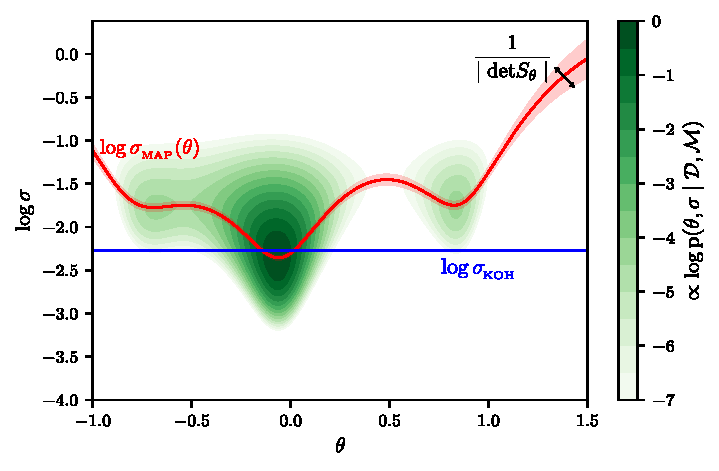
\includegraphics[width=\textwidth]{figures/cmp/fig_5.pdf}
    \caption{Slice of the un-normalized posterior distribution with $\sigma_e=0.01$ and $l=0.1$ (\gls{map} value of the hyperparameters in red and the \gls{koh} value in blue). The light red background is proportional to the magnitude of the inverse of the correction factor.}
    \label{fig:cmp:fig_5}
\end{figure}

Fig.~\ref{fig:cmp:fig_5} shows a slice of the resulting un-normalized posterior distribution, obtained by fixing two hyperparameters: the measurement noise $\sigma_e=0.01$ and the correlation length $l=0.1$. The red line shows the \gls{map} value of the hyperparameters, with variations representative of the scale of the inverse of the correction factor $\abs{\detf{\Stheta}}$, and the blue line shows the \gls{koh} value. This figure illustrates how different modular approaches simplify the resulting distribution by evaluating it along a single line in the case of the \gls{koh} method, or along a curve for the \gls{cmp} and \gls{fmp} methods. The posterior has two modes corresponding to $\theta \approx -0.1, 0.9$ with the second mode being less significant. The \gls{koh} method misses this second mode because its evaluation line does not pass through it. While other sequential approaches might provide better approximations, they are not guaranteed to capture all explanations accurately. 

\smallskip
As expected, not including the correction factor underestimates the effect of the tails, leading to a false certitude effect. This can be inferred from Fig.~\ref{fig:cmp:fig_5} by observing the relative scale of the correction factor, $\abs{\detf{\Stheta}}$, which increases at the tails.

\begin{figure}[htbp]
    \centering
    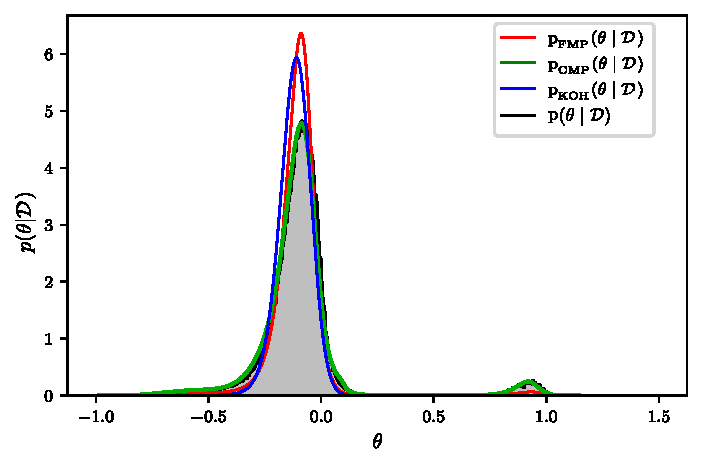
\includegraphics[width=\textwidth]{figures/cmp/fig_6.pdf}
    \caption{Posterior distribution computed using different approximation techniques. The histogram corresponds to samples from the \gls{fb} posterior.}
    \label{fig:cmp:fig_6}
\end{figure}

Fig.~\ref{fig:cmp:fig_6} presents the results of the calibration. It shows that the posterior has two modes at $\theta \approx -0.1$ and $\theta \approx 0.9$, with the second mode being more significant. The \gls{koh} approximation completely misses the second mode and exhibits the false certitude effect previously mentioned. The \gls{fmp} method captures both modes but significantly overestimates the weight of the first mode and also displays a similar false certitude effect. In contrast, the \gls{cmp} approximation provides an excellent approximation of the true posterior. 

\begin{figure}[htbp]
  \subfloat[Hyperparameters (\gls{map} in red and \gls{koh} in blue)\label{fig:cmp:fig_7a}]{
	\begin{minipage}[c]{0.50\textwidth}
	   \centering
	   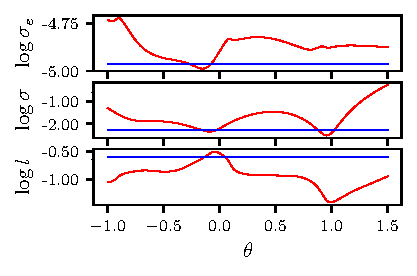
\includegraphics{figures/cmp/fig_7a.pdf}
	\end{minipage}}
 \hfill 	
  \subfloat[Correction factor\label{fig:cmp:fig_7b}]{
	\begin{minipage}[c]{0.50\textwidth}
	   \centering
	  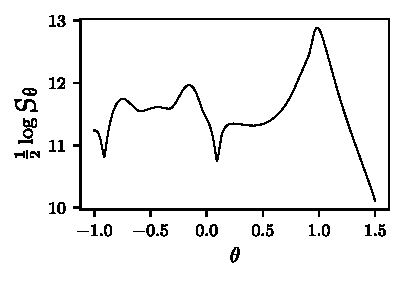
\includegraphics{figures/cmp/fig_7b.pdf}
	\end{minipage}}
\caption{Hyperparameters and correction factor used by the modular approaches.}
\label{fig:cmp:fig_7}
\end{figure}

Fig.~\ref{fig:cmp:fig_7} reports the value of the hyperparameters and the Hessian used by the \gls{cmp} method. The hyperparameters, see Fig.~\ref{fig:cmp:fig_7a}, used by the \gls{koh} method correspond to the average value, computed with respect to the final posterior distribution (see Eq.~\eqref{eq:koh_hpar}), of the ones used by the \gls{fmp}/\gls{cmp} methods. Their values will therefore be influenced by the presence of a strong peak around $\theta \approx -0.1$. The magnitude of the correction factor, depicted in Fig.~\ref{fig:cmp:fig_7b}, is significant. However, it is important to focus on relative variations rather than the absolute scale, as the \gls{cmp} method's approximation is valid up to a multiplicative constant. It is nevertheless interesting to observe that not including the Hessian would lead to a significant overestimation of the second mode. 

\subsection{Example 2: Higher Dimensional Uni-Modal Distribution}
\label{sc:cmp:test_case}

In this section, we will calibrate a model that relates the drag coefficient, $C_D$, of a smooth sphere moving through a fluid to its Reynolds number, Re. The first comprehensive characterization of this relationship was provided by Lapple and Shepherd in 1940 \cite{lapple_1940}, and is commonly referred to as the standard drag curve.
The current literature offers a wide range of tabulated experimental data and models, most of which are derived from empirical correlations. For a recent review of these resources, the interested reader is referred to \cite{gossens_2019}.

\smallskip
For simplicity, this work will utilize only the experimental data from \cite{lapple_1940}, which pertains to Reynolds numbers below 200,000, prior to the transition from laminar to fully turbulent flow. The model to be calibrated is based on the modified Stokes law (Eq.~8 in \cite{gossens_2019}) and depends on three parameters:

\begin{equation}
    C_D = \dfrac{A}{\text{Re}^B} + C \; .
    \label{eq:cmp:cd_model}
\end{equation}

\smallskip
For each tested method, the posterior distribution was sampled using an \gls{mcmc} algorithm. The parameter space has a dimensionality of 3, and we included a model error term with zero mean and a \gls{rbf} covariance as the covariance function, along with an experimental error term. This results in a total of 3 hyperparameters, bringing the overall dimensionality to 6.

\smallskip
The priors for the model parameters are uniform, while a set of inverse-gamma functions, detailed in Tab.~\ref{tab:cmp:hpar}, is used for the hyperparameters. 

\begin{table}[htbp]
    \centering 
    \begin{tabular}{|p{5em} || c | c ||  c | c |}
    \hline
        \textbf{Variable}  & $\alpha$ & $\beta$ & \textbf{mean} & \textbf{mode} \\
    \hline \hline
    $\sigma_e$ & 4 & 0.15 & 0.05 & 0.03\\ 
    $\sigma$  & 3 & 0.2& 0.1 & 0.05\\ 
    $l$ & 3 & 4 & 2 & 1\\ 
    \hline
    \end{tabular}
    \\[10pt]
    \caption{Parameters of the inverse-gamma priors of the hyperparameters and the corresponding mean and mode of the distribution.}
    \label{tab:cmp:hpar}
\end{table}


Inverse gamma priors are a popular choice of hyperparameter prior as they are conjugate priors for scale parameters \cite{uq_theory} and assign zero probability mass to unwanted events, such as zero, infinite, or negative values. The mean and mode of the inverse gamma distribution were chosen in order to separate the model and experimental errors'  strengths and to ensure that the correlation length is larger than the length scale of the experimental data.

\smallskip
We choose to perform the calibration of the $\log C_D$ versus $\log \text{Re}$ to account for the different orders of magnitude achieved by Eq.~\eqref{eq:cmp:cd_model}. 

\bigskip
A \gls{kde} of the posterior distribution is constructed using 10,000 independent samples. Independence is ensured by increasing the subsampling ratio to make it compatible with the correlation length.

\smallskip
For the \gls{fmp} method, the \gls{mcmc} chains for the posterior distribution were unable to reach convergence, in the sense of \cite{roy2019_MCMC}. This happens because the prior of the hyperparameters is not present in the \gls{fmp} approximation, making the resulting posterior distribution inaccurate and difficult to sample from. In \cite{fmp} the authors use only uniform distributions for the prior of the hyperparameters hence this problem does not appear.

\begin{figure}[htbp]
    \centering
    
    % --- Row 1 ---
    \begin{subfigure}[t]{0.49\textwidth}
        \centering
        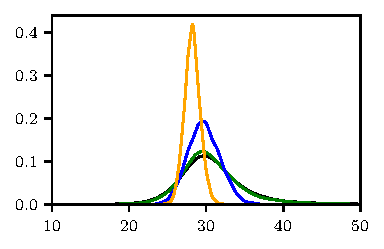
\includegraphics[width=\textwidth]{figures/cmp/fig_8a.pdf}
        \caption{The posterior distribution of $A$}
        \label{fig:cmp:8a}
    \end{subfigure}% <--- THIS % IS CRITICAL. DO NOT REMOVE IT.
    \hfill
    \begin{subfigure}[t]{0.49\textwidth}
        \centering
        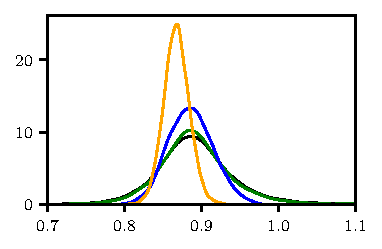
\includegraphics[width=\textwidth]{figures/cmp/fig_8b.pdf}
        \caption{The posterior distribution of $B$}
        \label{fig:cmp:8b}
    \end{subfigure}
    
    \vspace{1em} % Adds vertical space between the two rows
    
    % --- Row 2 ---
    \begin{subfigure}[t]{0.48\textwidth}
        \centering
        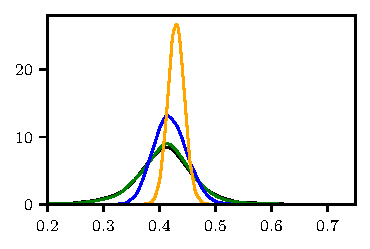
\includegraphics[width=\textwidth]{figures/cmp/fig_8c.pdf}
        \caption{The posterior distribution of $C$}
        \label{fig:cmp:8c}
    \end{subfigure}%  <--- THIS % IS CRITICAL. DO NOT REMOVE IT.
    \hfill
    \begin{subfigure}[t]{0.48\textwidth}
        \centering
        \raisebox{1.5cm}{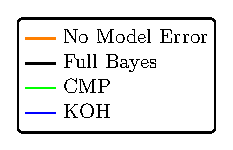
\includegraphics[width=0.5\textwidth]{figures/cmp/fig_8d.eps}}
        \label{fig:cmp:8d}
    \end{subfigure}
    
    \caption{Comparison between different approximations of the marginal posterior.}
    \label{fig:cmp:fig_8}
\end{figure}

\begin{table}[htbp]
    \centering 
    \begin{tabular}{|p{5em} || c | c || c | c || c | c |}
    \hline
          & \multicolumn{2}{c ||}{A} & \multicolumn{2}{c ||}{B} & \multicolumn{2}{c |}{C} \\
        \hline
        \textbf{Parameter} & $\mu$ & $\sigma$ & $\mu$ & $\sigma$ & $\mu$ & $\sigma$ \\
    \hline \hline
    %BAYES & $31.2 \pm 0.14$ & $6.87 \pm 0.73$ & $0.89 \pm 0.01$ & $0.054 \pm 0.001$ & $0.41 \pm 0.001$ & $0.07 \pm 0.005$ \\
    %\gls{cmp}   & $30.9 \pm 0.11$ & $5.65 \pm 0.44$ & $0.89 \pm 0.01$ & $0.050 \pm 0.001$ & $0.41 \pm 0.001$ & $0.06 \pm 0.003$ \\
    %\gls{koh}   & $29.7 \pm 0.04$ & $2.09 \pm 0.03$ & $0.89 \pm 0.01$ & $0.029 \pm 0.001$ & $0.41 \pm 0.001$ & $0.03 \pm 0.001$ \\

    BAYES & $31.2$ & $6.87$ & $0.89$ & $0.054$ & $0.41$ & $0.07$ \\
    \gls{cmp}   & $30.9$ & $5.65$ & $0.89$ & $0.050$ & $0.41$ & $0.06$ \\
    \gls{koh}   & $29.7$ & $2.09$ & $0.89$ & $0.029$ & $0.41$ & $0.03$ \\
    \hline
    \end{tabular}
    \\[10pt]
    \caption{Mean and variance of the parameters.}
    \label{tab:cmp:mean_var_par}
\end{table}

Fig.~\ref{fig:cmp:fig_8} reports the approximation of the marginal posterior distribution of the parameters computed using the three different methods along with the one computed without the model error term. The latter was included to justify the inclusion of the model error since the resulting distribution is too overconfident and explains all errors as measurement noise. The mean and standard deviations of the marginal posteriors are also reported in Tab.~\ref{tab:cmp:mean_var_par}. Both the table and the \gls{kde} plot show that the \gls{koh} method underestimates the variance of the distribution by more than 50 \%. The \gls{cmp} estimation of the variance, on the other hand, is much closer to the \gls{fb} one. This agrees with the previous discussion and is due to two contributions. First and foremost, the variable model error term can consider more explanations and the correction factor increases the weight of the tails, where the residual is larger.


\begin{figure}[htbp]
    \centering
    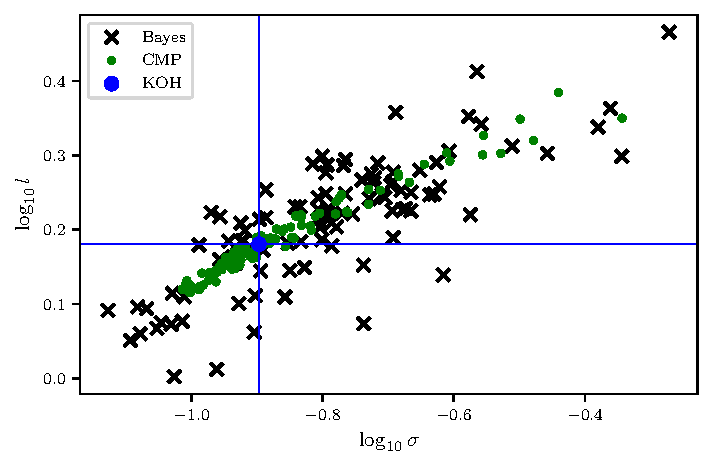
\includegraphics[width=\textwidth]{figures/cmp/fig_9.pdf}
    \caption{Joint plot of the covariance strength, $\sigma$, and the correlation length, $l$.}
    \label{fig:cmp:fig_9}
\end{figure}

Fig.~\ref{fig:cmp:fig_9} shows the joint plot of the two hyperparameters that characterize the model error covariance. For the \gls{fb} approach, the samples shown correspond to samples extracted from the marginal posterior of the hyperparameters, $\p{\bpsi \mid \data}$. For the \gls{cmp} case, they are samples of $\psimap$ where $\btheta \sim \approxp{\cmp}{\btheta \mid \data}$ and the blue dot is the \gls{koh} value. This shows that non-sequential methods yield a model error term that has a richer structure than the one computed by sequential approaches. An interesting correlation between these two hyperparameters can also be noted: larger model error corrections (larger $\sigma$) necessitate longer correlation lengths. 

\begin{figure}[htbp]
    \centering
    
    % --- Row 1 ---
    \begin{subfigure}[t]{0.48\textwidth}
        \centering
        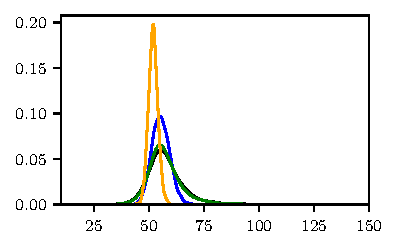
\includegraphics[width=\textwidth]{figures/cmp/fig_10a.pdf}
        \caption{$C_D$ for Re=0.5}
        \label{fig:cmp:10a}
    \end{subfigure}% <--- Critical % to prevent line break
    \hfill  
    \begin{subfigure}[t]{0.48\textwidth}
        \centering
        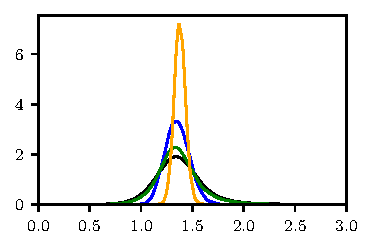
\includegraphics[width=\textwidth]{figures/cmp/fig_10b.pdf}
        \caption{$C_D$ for Re=50}
        \label{fig:cmp:10b}
    \end{subfigure}
    
    \vspace{1.5em} % Spacing between rows
    
    % --- Row 2 ---
    \begin{subfigure}[t]{0.48\textwidth}
        \centering
        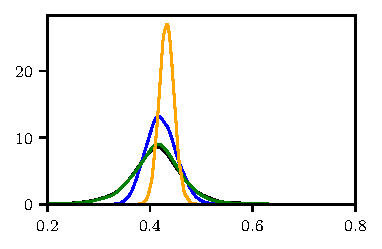
\includegraphics[width=\textwidth]{figures/cmp/fig_10c.pdf}
        \caption{$C_D$ for Re=50,000}
        \label{fig:cmp:10c}
    \end{subfigure}% <--- Critical % to prevent line break
    \hfill
    \begin{subfigure}[t]{0.48\textwidth}
        \centering
        \raisebox{1.5cm}{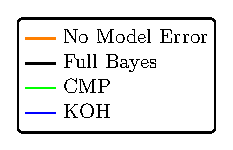
\includegraphics[width=0.5\textwidth]{figures/cmp/fig_10d.eps}}
        \label{fig:cmp:10d}
    \end{subfigure}
    
    \caption{Predictive distribution of the calibrated model.}
    \label{fig:cmp:fig_10}
\end{figure}

The predictive distribution without considering the model error correction, computed using the different approximations, is reported in Fig.~\ref{fig:cmp:fig_10} for three values of the Reynolds number. The latter are considered representative of different scales; looking at Eq.~\eqref{eq:cmp:cd_model}, the first value of Re is very small so the non-constant term dominates, the second one is an intermediate value, and at the third one, the constant term dominates.

\smallskip
As visible from Fig.~\ref{fig:cmp:fig_10}, not considering the model error or using a sequential approach has a large impact on the robustness of the posterior prediction as the results are too overconfident. Again, the \gls{cmp} approximation is revealed to be an excellent one.

\begin{figure}[htbp]
    \centering
    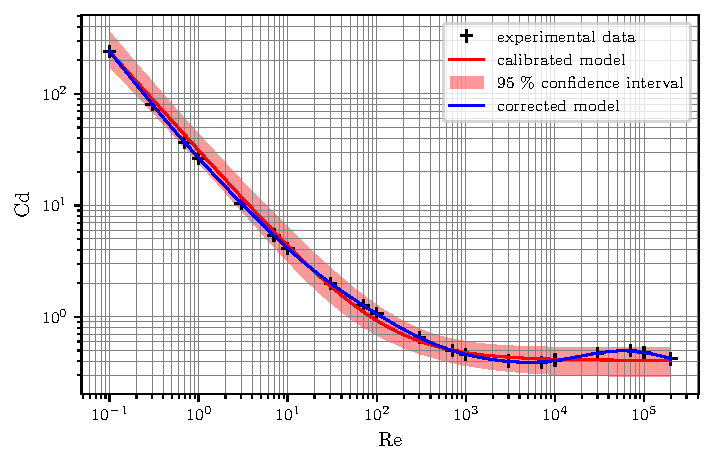
\includegraphics[width=\textwidth]{figures/cmp/fig_11.pdf}
    \caption{\gls{cmp} prediction}
    \label{fig:cmp:fig_11}
\end{figure}

Finally, Fig.~\ref{fig:cmp:fig_11} shows the predictive distribution for all Reynolds numbers in the observed interval. The figure contains also the mean value of the corrected model (see Eq.~\eqref{eq:cmp:corr_pred} and Eq.~\eqref{eq:cmp:corr_pred}) and the experimental data with the measurement noise. This shows that the model error can explain the discrepancy between the observed value and the model's computation; moreover, the standard deviation of the corrected model prediction is very small. The same plot reveals, however, that there might be a confounding issue between the model and experimental error. The inferred value of the standard deviation of the measurement noise is very small, on the order of $10^{-3}$, and the entire discrepancy is explained by the model error. This problem is intrinsic to the data and the model itself since the inferred value of the correction length is large, see Fig.~\ref{fig:cmp:fig_9}, and hence there is no confusion between the structure of the experimental error (which is un-correlated) and the one of the model error (whose correction length spans more than one order of magnitude). This confounding issue could be solved by using more data, possibly more $\log C_D$ measurements for each $\log \text{Re}$ value. 

\section{Conclusions}
\label{sc:conc}

In this chapter, we have introduced a novel approach to solving the calibration problem with the inclusion of model error. The new \gls{cmp} method is based on the Bayesian calibration framework for estimating model parameters and model error hyperparameters. This method advances the current state of the art by providing a closed-form approximation of the parameters' marginal posterior distribution, effectively eliminating the need to sample the model error hyperparameters. This approximation surpasses those provided by other modular approaches, such as the \gls{koh} and \gls{fmp} methods, as it consistently accounts for the uncertainty of the hyperparameters. Compared to the reference \gls{fb} approach, the \gls{cmp} method offers an excellent approximation.

\smallskip
To achieve this, we formulated a new set of assumptions on the posterior distribution that are less stringent and more general. These assumptions systematically account for the possibility that conditioning the posterior distribution on different parameter values can result in conditional distributions of the hyperparameters with varying means and variances but constant shapes. Given a specific calibration problem, it seems difficult to verify a priori whether the hypotheses of the \gls{cmp} method are respected. However, an a posteriori verification can be performed for a few parameter values by sampling the hyperparameters' conditional distribution and assessing the assumption that all samples come from the same distribution up to scale-shift transformations.

We tested the \gls{cmp} method with two theoretical examples. In one example, we assumed the posterior distribution could be represented as a mixture of Gaussians with different means and variances. Here, the \gls{cmp} approximation provided the exact answer, whereas other popular approaches either failed to capture all modes or assigned incorrect weights to them. In the other example, we examined the calibration problem without model error, where experimental noise was the only hyperparameter. Again, the \gls{cmp} approximation was exact, while popular modular approaches suffered from a false certitude effect, assigning less weight to the distribution tails.

Additionally, we demonstrated the effectiveness of the \gls{cmp} method with two numerical examples. In the first, targeting a 1D bimodal distribution, the \gls{cmp} method accurately identified both modes and their weights, similar to the Gaussian mixture case. In the second example, focusing on a higher-dimensional unimodal distribution, the \gls{cmp} method avoided the false certitude effect and provided an excellent approximation of the MAP value and its uncertainty.

\bigskip
At this stage, the \gls{cmp} method still relies on the solution of a generally non-convex optimization problem to compute the optimal hyperparameters, $\psimap$. This can be a computationally expensive task, especially if the number of hyperparameters is large. Furthermore, in \gls{mcmc} sampling, querying $\psimap$ is required at each step, compounding the computational cost. The next chapter is dedicated to addressing this issue by introducing a surrogate model for $\psimap$ to significantly reduce the computational burden.